\begin{tabular}[ht]{cccccN}
  \hline
  \multicolumn{2}{c}{Number of particles} & Position of particles in cell $c$ & Euler CFL & RK2 CFL &\\[6pt]
  \hline
  \hline
  1 &(--) &$x_1 \in \[x_{2c-1},x_{2c}\]$  & 1.00& 1.00&\\[8pt]
  \hline
  2 &(i)& 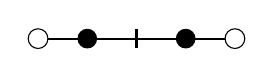
\begin{tikzpicture}[scale=2.5]
             \draw[thick] (0,0) -- (1.,0);
             \draw[thick] (0.5,-0.05) -- (0.5,0.05);
             \fill[white] (0,0) circle (0.05);\draw (0,0) circle (0.05);
             \fill[white] (1.,0) circle (0.05);\draw (1,0) circle (0.05);
             \fill[black] (0.25,0) circle (0.05);\fill[black] (0.75,0) circle (0.05);
           \end{tikzpicture} &  0.43 & 1.00&\\[8pt]
  % 2PPC shifted
  2& (ii)&  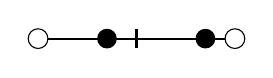
\begin{tikzpicture}[scale=2.5]
             \draw[thick] (0,0) -- (1.,0);
             \draw[thick] (0.5,-0.05) -- (0.5,0.05);
             \fill[white] (0,0) circle (0.05);\draw (0,0) circle (0.05);
             \fill[white] (1.,0) circle (0.05);\draw (1,0) circle (0.05);
             \fill[black] (0.25+0.1,0) circle (0.05);\fill[black] (0.75+0.1,0) circle (0.05);
           \end{tikzpicture}  &  0.40 & 0.50 &\\[8pt]
  % 2PPC shifted left on nodes
  2 & (iii)& 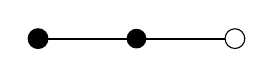
\begin{tikzpicture}[scale=2.5]
             \draw[thick] (0,0) -- (1.,0);
             \draw[thick] (0.5,-0.05) -- (0.5,0.05);
             \fill[white] (0,0) circle (0.05);\draw (0,0) circle (0.05);
             \fill[white] (1.,0) circle (0.05);\draw (1,0) circle (0.05);
             \fill[black] (0.,0) circle (0.05);\fill[black] (0.5,0) circle (0.05);
           \end{tikzpicture}  &  0.50 & 0.61 &\\[8pt]
  % 2PPC shifted right on nodes
  2 & (iv)& 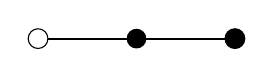
\begin{tikzpicture}[scale=2.5]
             \draw[thick] (0,0) -- (1.,0);
             \draw[thick] (0.5,-0.05) -- (0.5,0.05);
             \fill[white] (0,0) circle (0.05);\draw (0,0) circle (0.05);
             \fill[white] (1.,0) circle (0.05);\draw (1,0) circle (0.05);
             \fill[black] (0.5,0) circle (0.05);\fill[black] (1,0) circle (0.05);
           \end{tikzpicture}  &  0.30 & 0.31 &\\[8pt]
  % 2PPC shifted symmetrical
  2 & (v)& 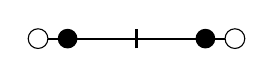
\begin{tikzpicture}[scale=2.5]
             \draw[thick] (0,0) -- (1.,0);
             \draw[thick] (0.5,-0.05) -- (0.5,0.05);
             \fill[white] (0,0) circle (0.05);\draw (0,0) circle (0.05);
             \fill[white] (1.,0) circle (0.05);\draw (1,0) circle (0.05);
             \fill[black] (0.25-0.1,0) circle (0.05);\fill[black] (0.75+0.1,0) circle (0.05);
           \end{tikzpicture}  &  0.27 &1.00&\\[8pt]
  % 2PPC shifted symmetrical on nodes
  2 & (vi)& 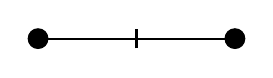
\begin{tikzpicture}[scale=2.5]
             \draw[thick] (0,0) -- (1.,0);
             \draw[thick] (0.5,-0.05) -- (0.5,0.05);
             \fill[white] (0,0) circle (0.05);\draw (0,0) circle (0.05);
             \fill[white] (1.,0) circle (0.05);\draw (1,0) circle (0.05);
             \fill[black] (0.,0) circle (0.05);\fill[black] (1.,0) circle (0.05);
           \end{tikzpicture}  &  0.00 & 1.00 &\\[8pt]
  \hline
  % 3PPC 
  3 & (i)& 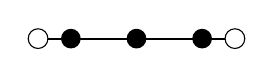
\begin{tikzpicture}[scale=2.5]
             \draw[thick] (0,0) -- (1.,0);
             \draw[thick] (0.5,-0.05) -- (0.5,0.05);
             \fill[white] (0,0) circle (0.05);\draw (0,0) circle (0.05);
             \fill[white] (1.,0) circle (0.05);\draw (1,0) circle (0.05);
             \fill[black] (1./6.,0) circle (0.05);\fill[black] (0.5,0) circle (0.05);
             \fill[black] (1.-1./6.,0) circle (0.05);
           \end{tikzpicture} &  0.30 & 1.00&\\[8pt]
  % 3PPC shifted
  3&  (ii)&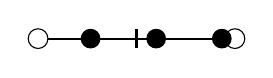
\begin{tikzpicture}[scale=2.5]
             \draw[thick] (0,0) -- (1.,0);
             \draw[thick] (0.5,-0.05) -- (0.5,0.05);
             \fill[white] (0,0) circle (0.05);\draw (0,0) circle (0.05);
             \fill[white] (1.,0) circle (0.05);\draw (1,0) circle (0.05);
             \fill[black] (1./6.+0.1,0) circle (0.05);\fill[black] (0.5+0.1,0) circle (0.05);
             \fill[black] (1.-1./6.+0.1,0) circle (0.05);
           \end{tikzpicture} &  0.26 & 0.06 &\\[8pt]
  % 3PPC shifted left on nodes
  3 & (iii)&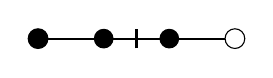
\begin{tikzpicture}[scale=2.5]
             \draw[thick] (0,0) -- (1.,0);
             \draw[thick] (0.5,-0.05) -- (0.5,0.05);
             \fill[white] (0,0) circle (0.05);\draw (0,0) circle (0.05);
             \fill[white] (1.,0) circle (0.05);\draw (1,0) circle (0.05);
             \fill[black] (0,0) circle (0.05);
             \fill[black] (0.5-1/6,0) circle (0.05);
             \fill[black] (1.-2./6.,0) circle (0.05);
           \end{tikzpicture} &  0.33 & 0.73 &\\[8pt]
  % 3PPC shifted right on nodes
  3 & (iv)&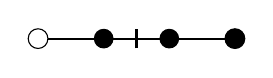
\begin{tikzpicture}[scale=2.5]
             \draw[thick] (0,0) -- (1.,0);
             \draw[thick] (0.5,-0.05) -- (0.5,0.05);
             \fill[white] (0,0) circle (0.05);\draw (0,0) circle (0.05);
             \fill[white] (1.,0) circle (0.05);\draw (1,0) circle (0.05);
             \fill[black] (1./3.,0) circle (0.05);
             \fill[black] (0.5+1./6.,0) circle (0.05);
             \fill[black] (1,0) circle (0.05);
           \end{tikzpicture} &  0.22 & 0.17 &\\[8pt]
  % 3PPC symmetrical
  3 &(v) & 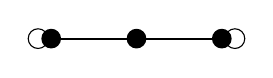
\begin{tikzpicture}[scale=2.5]
             \draw[thick] (0,0) -- (1.,0);
             \draw[thick] (0.5,-0.05) -- (0.5,0.05);
             \fill[white] (0,0) circle (0.05);\draw (0,0) circle (0.05);
             \fill[white] (1.,0) circle (0.05);\draw (1,0) circle (0.05);
             \fill[black] (1./6.-0.1,0) circle (0.05);\fill[black] (0.5+0.,0) circle (0.05);
             \fill[black] (1.-1./6.+0.1,0) circle (0.05);
           \end{tikzpicture} &  0.13 & 1.00 &\\[8pt]
  % 3PPC symmetrical on nodes
  3& (vi)& 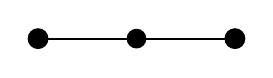
\begin{tikzpicture}[scale=2.5]
             \draw[thick] (0,0) -- (1.,0);
             \draw[thick] (0.5,-0.05) -- (0.5,0.05);
             \fill[white] (0,0) circle (0.05);\draw (0,0) circle (0.05);
             \fill[white] (1.,0) circle (0.05);\draw (1,0) circle (0.05);
             \fill[black] (0.,0) circle (0.05);\fill[black] (0.5,0) circle (0.05);
             \fill[black] (1,0) circle (0.05);
           \end{tikzpicture} &  0.00 & 1.00 &\\[8pt]
  \hline
  % 4PPC 
  4 & (i)& 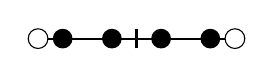
\begin{tikzpicture}[scale=2.5]
             \draw[thick] (0,0) -- (1.,0);
             \draw[thick] (0.5,-0.05) -- (0.5,0.05);
             \fill[white] (0,0) circle (0.05);\draw (0,0) circle (0.05);
             \fill[white] (1.,0) circle (0.05);\draw (1,0) circle (0.05);
             \fill[black] (0.125,0) circle (0.05);\fill[black] (0.375,0) circle (0.05);
             \fill[black] (0.625,0) circle (0.05);\fill[black] (0.875,0) circle (0.05);
           \end{tikzpicture} &  0.23 & 1.00&\\[8pt]
  % 4PPC shifted
  4 &(ii) & 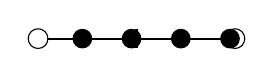
\begin{tikzpicture}[scale=2.5]
             \draw[thick] (0,0) -- (1.,0);
             \draw[thick] (0.5,-0.05) -- (0.5,0.05);
             \fill[white] (0,0) circle (0.05);\draw (0,0) circle (0.05);
             \fill[white] (1.,0) circle (0.05);\draw (1,0) circle (0.05);
             \fill[black] (0.125+0.1,0) circle (0.05);\fill[black] (0.375+0.1,0) circle (0.05);
             \fill[black] (0.625+0.1,0) circle (0.05);\fill[black] (0.875+0.1,0) circle (0.05);
           \end{tikzpicture} &  0.20 & 0.16 &\\[8pt]
  % 4PPC shifted left on nodes
  4 & (iii)&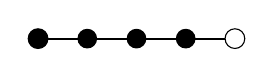
\begin{tikzpicture}[scale=2.5]
             \draw[thick] (0,0) -- (1.,0);
             \draw[thick] (0.5,-0.05) -- (0.5,0.05);
             \fill[white] (0,0) circle (0.05);\draw (0,0) circle (0.05);
             \fill[white] (1.,0) circle (0.05);\draw (1,0) circle (0.05);
             \fill[black] (0.125-1./8.,0) circle (0.05);\fill[black] (0.375-1./8.,0) circle (0.05);
             \fill[black] (0.625-1./8.,0) circle (0.05);\fill[black] (0.875-1./8.,0) circle (0.05);
           \end{tikzpicture} &  0.25 & 0.79 &\\[8pt]
  % 4PPC shifted right on nodes
  4 & (iv)&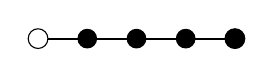
\begin{tikzpicture}[scale=2.5]
             \draw[thick] (0,0) -- (1.,0);
             \draw[thick] (0.5,-0.05) -- (0.5,0.05);
             \fill[white] (0,0) circle (0.05);\draw (0,0) circle (0.05);
             \fill[white] (1.,0) circle (0.05);\draw (1,0) circle (0.05);
             \fill[black] (0.125+1./8.,0) circle (0.05);\fill[black] (0.375+1./8.,0) circle (0.05);
             \fill[black] (0.625+1./8.,0) circle (0.05);\fill[black] (0.875+1./8.,0) circle (0.05);
           \end{tikzpicture} &  0.18 & 0.11 &\\[8pt]
  % 4PPC symmetrical
  4 & (v)&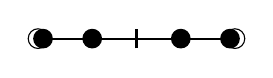
\begin{tikzpicture}[scale=2.5]
             \draw[thick] (0,0) -- (1.,0);
             \draw[thick] (0.5,-0.05) -- (0.5,0.05);
             \fill[white] (0,0) circle (0.05);\draw (0,0) circle (0.05);
             \fill[white] (1.,0) circle (0.05);\draw (1,0) circle (0.05);
             \fill[black] (0.125-0.1,0) circle (0.05);\fill[black] (0.375-0.1,0) circle (0.05);
             \fill[black] (0.625+0.1,0) circle (0.05);\fill[black] (0.875+0.1,0) circle (0.05);
           \end{tikzpicture} &  0.05 & 1.00 &\\[8pt]
  % 4PPC symmetrical on nodes
  4 & (vi)&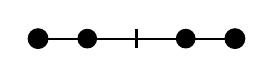
\begin{tikzpicture}[scale=2.5]
             \draw[thick] (0,0) -- (1.,0);
             \draw[thick] (0.5,-0.05) -- (0.5,0.05);
             \fill[white] (0,0) circle (0.05);\draw (0,0) circle (0.05);
             \fill[white] (1.,0) circle (0.05);\draw (1,0) circle (0.05);
             \fill[black] (0.125-1./8.,0) circle (0.05);\fill[black] (0.375-1./8.,0) circle (0.05);
             \fill[black] (0.625+1./8.,0) circle (0.05);\fill[black] (0.875+1./8.,0) circle (0.05);
           \end{tikzpicture} &  0.00 & 1.00 &\\[8pt]
  \hline
\end{tabular}

%%% Local Variables: 
%%% mode: latex
%%% TeX-master: "../manuscript"
%%% End: